\section{第四章 连续信息的度量}

\begin{remarkBox}{本章重点}
前两章处理的是离散信源——符号可数，概率求和。从这一章开始，信源的输出变成连续随机变量，信息度量的工具也从离散熵过渡到差熵。学习时先抓住「离散化取极限」这个核心思想，再掌握高斯分布的熵公式和最大熵定理，最后把差熵与互信息的关系和前两章的结论衔接起来。
\end{remarkBox}

\subsection{连续随机变量集合的熵}

\subsubsection{连续随机变量的离散化}
连续信源不能直接套用离散熵的求和公式，因为连续取值点在实数轴上是稠密的。信息论的处理方法是：先把连续随机变量划分成等间距的小区间，算出离散化后的熵，再让区间宽度趋于零取极限。

\begin{definitionBox}{连续随机变量的离散化}
设连续随机变量 $X$ 的概率密度为 $p(x)$。将 $X$ 的取值区间划分为宽为 $\Delta x$ 的等间隔小区间 $\{S_i\}$，在每个小区间内取代表点 $x_i$，则离散化后的概率近似为
\[
P(x_i)\approx p(x_i)\Delta x.
\]
\end{definitionBox}

这是一种「先离散再取极限」的策略——本章所有连续信息度量的定义都建立在这个基础之上。

\subsubsection{差熵的定义}

\begin{definitionBox}{差熵（Differential Entropy）}
连续随机变量 $X$ 的差熵定义为
\[
h(X)=-\int_{\mathbb{R}}p(x)\log p(x)\,\mathrm{d}x
      =E\{-\log p(x)\}.
\]
单位：比特（或奈特）/ 自由度。
\end{definitionBox}

\begin{warningBox}{差熵不是绝对度量}
离散化后信源的熵包含两项：一项是 $\lim_{\Delta x\to 0}(-\log\Delta x)$，它是无穷大的「绝对熵」，与分布无关；另一项才是差熵。因此差熵只能作为\textbf{相对}的比较工具——差熵大的信源平均不确定性更大，但它本身可以是负值。
\end{warningBox}

\subsubsection{联合差熵与条件差熵}

类似离散情形，可以把差熵推广到多维：

\begin{definitionBox}{联合差熵}
$N$ 维连续随机矢量 $X^N=(X_1,\dots,X_N)$ 的联合差熵为
\[
h(X^N)=-\int_{\mathbb{R}^N} p(\bm{x})\log p(\bm{x})\,\mathrm{d}\bm{x}
      =E\{-\log p(\bm{x})\}.
\]
单位：比特 / $N$ 自由度。
\end{definitionBox}

\begin{definitionBox}{条件差熵}
给定 $Y$ 时 $X$ 的条件差熵为
\[
h(X\mid Y)=-\iint_{\mathbb{R}^2} p(x,y)\log p(x\mid y)\,\mathrm{d}x\mathrm{d}y.
\]
\end{definitionBox}

\subsubsection{差熵的性质}

差熵保持了离散熵的大部分结构性规律，但有三点关键差异。

\begin{formulaBox}{差熵的可加性}
对 $N$ 维随机矢量 $X^N$，
\[
h(X^N)=h(X_1)+h(X_2\mid X_1)+\cdots+h(X_N\mid X_1\cdots X_{N-1})
      \le \sum_{i=1}^N h(X_i),
\]
仅当各分量独立时取等号。
\end{formulaBox}

\begin{formulaBox}{线性变换下的差熵}
设 $Y=AX+\bm{\alpha}$，其中 $A$ 为 $N\times N$ 可逆矩阵，则
\[
h(Y)=h(X)+\log|\det(A)|.
\]
\textbf{直觉理解}：$\det(A)$ 是线性变换 $A$ 对 $N$ 维体积的缩放因子。如果 $|\det(A)|>1$，变换把概率密度「撑开」了——原本挤在一起的样本点被拉开，不确定性增大，熵增加 $\log|\det(A)|$。反之，若变换是压缩的（$|\det(A)|<1$），熵会减少。

特别地，若 $A$ 为正交矩阵（旋转/反射），则 $\det(A)=\pm1$，$h(Y)=h(X)$——平移和旋转不改变差熵。
\end{formulaBox}

差熵与离散熵的关键差异包括：
\begin{itemize}
  \item 差熵\textbf{不一定是非负的}：概率密度可能大于 1，导致 $-\log p(x)<0$。
  \item 差熵\textbf{在非线性变换下可能改变}：只有线性变换有简洁的加减规律。
  \item 差熵是\textbf{相对量度}，不能直接比较不同量纲的信源（如电压和温度）。
\end{itemize}

\subsubsection{连续随机变量的相对熵}

\begin{definitionBox}{连续相对熵（KL 散度）}
设 $p(x)$ 和 $q(x)$ 为同一空间上的两个概率密度，定义 $p$ 相对于 $q$ 的散度为
\[
D(p\|q)=\int_{\mathbb{R}} p(x)\log\frac{p(x)}{q(x)}\,\mathrm{d}x.
\]
\end{definitionBox}

\begin{theoremBox}{散度不等式（定理 4.2）}
$D(p\|q)\ge 0$，当且仅当 $p(x)=q(x)$ 几乎处处成立时取等号。
\end{theoremBox}

\subsection{离散时间高斯随机变量集合的熵}

高斯分布在连续信源中占据核心地位——它不仅是自然界最常见的分布，也是最大熵定理的主角。

\subsubsection{一维高斯随机变量的熵}

\begin{theoremBox}{一维高斯熵（定理 4.1）}
设 $X\sim\mathcal{N}(m,\sigma^2)$，则
\[
h(X)=\frac{1}{2}\log(2\pi e\sigma^2).
\]
高斯信源的熵仅与方差有关，与均值无关——均值只影响分布的中心位置，不影响散布程度。

\noindent \textbf{常数 $2\pi e$ 的含义}：$\pi$ 来自高斯密度归一化常数中的 $\sqrt{2\pi\sigma^2}$，$e$ 来自指数项 $\exp(-x^2/2\sigma^2)$ 取对数后产生的二次项。若用自然对数，则 $\log e=1$；若用以 2 为底的对数，则对应结果以 bit 为单位。记住「$\log\sigma^2$ + 常数」这个结构就够了——方差翻倍时，差熵增加 $\frac12\log 2$，其单位由对数底决定。
\end{theoremBox}

\begin{proof}
将 $p(x)=\frac{1}{\sqrt{2\pi\sigma^2}}\exp\bigl(-\frac{(x-m)^2}{2\sigma^2}\bigr)$ 代入 $h(X)=-E\{\log p(x)\}$：
\[
-\log p(x)=\frac{1}{2}\log(2\pi\sigma^2)+\frac{(x-m)^2}{2\sigma^2}\log e,
\]
取期望，$E\{(x-m)^2\}=\sigma^2$，得 $h(X)=\frac{1}{2}\log(2\pi e\sigma^2)$。
\end{proof}

\subsubsection{多维高斯随机矢量的熵}

\begin{theoremBox}{多维独立高斯矢量的熵}
设 $X^N=(X_1,\dots,X_N)$ 各分量独立，$X_i\sim\mathcal{N}(m_i,\sigma_i^2)$，则
\[
h(X^N)=\sum_{i=1}^N h(X_i)=\frac{N}{2}\log\bigl[2\pi e(\sigma_1^2\sigma_2^2\cdots\sigma_N^2)^{1/N}\bigr].
\]
\end{theoremBox}

\begin{theoremBox}{定理 4.3：多维相关高斯矢量的熵}
设 $X^N$ 服从 $N$ 维联合高斯分布，协方差矩阵为 $\Sigma$，则
\[
h(X^N)=\frac{N}{2}\log\bigl[2\pi e\det(\Sigma)^{1/N}\bigr].
\]

\noindent \textbf{从独立到相关}：如果各分量独立，$\Sigma$ 是对角矩阵，$\det(\Sigma)=\prod_i\sigma_i^2$，公式退化为独立情形的 $(N/2)\log[2\pi e(\prod\sigma_i^2)^{1/N}]$。一旦引入相关性，非对角元素使 $\det(\Sigma)$ 小于 $\prod\sigma_i^2$（因为相关性的存在使概率质量更集中），联合熵随之降低。$(\det\Sigma)^{1/N}$ 可以理解为「平均每个自由度的有效方差」。
\end{theoremBox}

\begin{keypoint}{相关性的影响}
比较独立情形和相关情形：独立时熵取决于 $\prod\sigma_i^2$，相关时取决于 $\det(\Sigma)$。由于 $\det(\Sigma)\le\prod\sigma_i^2$（Hadamard 不等式），相关性使联合熵降低——这和离散信源中「相关性越强熵越低」的规律完全一致。
\end{keypoint}

\begin{example}
\label{ex:gauss-linear-transform}
\textbf{线性变换下的高斯熵}：设独立高斯变量 $X\sim\mathcal{N}(m_x,\sigma_x^2)$，$Y\sim\mathcal{N}(m_y,\sigma_y^2)$，令 $U=X+Y$，$V=X-Y$。求 $h(U,V)$。

\noindent \textbf{解题流程}：\\[2pt]
步骤一：写出 $(U,V)$ 到 $(X,Y)$ 的线性变换。\\
步骤二：利用线性变换公式 $h(U,V)=h(X,Y)+\log|\det(A)|$。\\
步骤三：$X$、$Y$ 独立，$h(X,Y)=h(X)+h(Y)$。

\noindent \textbf{解}：\\[2pt]
变换矩阵 $\begin{pmatrix}U\\V\end{pmatrix}=\begin{pmatrix}1&1\\1&-1\end{pmatrix}\begin{pmatrix}X\\Y\end{pmatrix}$，$\det(A)=-2$，$|\det(A)|=2$。
\[
h(X,Y)=h(X)+h(Y)=\frac{1}{2}\log(2\pi e\sigma_x^2)+\frac{1}{2}\log(2\pi e\sigma_y^2)=\log(2\pi e\sigma_x\sigma_y).
\]
\[
h(U,V)=h(X,Y)+\log 2=\log(4\pi e\sigma_x\sigma_y).
\]
\end{example}

\begin{example}
\label{ex:gauss-orthogonal}
\textbf{正交变换下的高斯熵}：将上例改为 $U=\frac{X+Y}{\sqrt{2}}$，$V=\frac{X-Y}{\sqrt{2}}$，求 $h(U,V)$。

\noindent \textbf{解}：\\[2pt]
此时变换矩阵为正交矩阵，$\det(A)=\pm1$，故 $h(U,V)=h(X,Y)=\log(2\pi e\sigma_x\sigma_y)$。正交变换（旋转）不改变联合差熵，这一性质在信号处理中经常用到。
\end{example}

\subsection{连续最大熵定理}

离散信源在等概时熵最大。连续信源的「等概」对应均匀分布，但均匀分布只能在有限区间上定义——这就引出了两种约束下的最大熵定理。

\begin{theoremBox}{定理 4.4：限峰值最大熵定理（幅度受限）}
若随机变量 $X$ 的取值限定在区间 $[a,b]$ 内（峰值功率受限），则当 $X$ 在 $[a,b]$ 上\textbf{均匀分布}时差熵最大：
\[
h(X)\le\log(b-a).
\]
推广到 $N$ 维：$X^N$ 在超矩形 $\prod[a_i,b_i]$ 上均匀分布时熵最大，
\[
h(X^N)\le\sum_{i=1}^N\log(b_i-a_i).
\]
\end{theoremBox}

\begin{theoremBox}{定理 4.5：限平均功率最大熵定理（功率受限）}
若 $N$ 维随机矢量 $X^N$ 的协方差矩阵 $\Sigma$ 固定（平均功率受限），则当 $X^N$ 服从\textbf{联合高斯分布}时差熵最大：
\[
h(X^N)\le\frac{N}{2}\log\bigl[2\pi e\det(\Sigma)^{1/N}\bigr].
\]
特别地，一维情形（方差 $\sigma^2$ 受限）：$h(X)\le\frac{1}{2}\log(2\pi e\sigma^2)$，当 $X\sim\mathcal{N}(m,\sigma^2)$ 时取等号。若额外限定零均值，则写作 $X\sim\mathcal{N}(0,\sigma^2)$。
\end{theoremBox}

\begin{keypoint}{两个定理的直觉记忆}
\begin{itemize}
  \item \textbf{幅度受限} $\to$ \textbf{均匀分布}：不能超出范围，那就让每个位置「一样可能」——这和离散信源等概时熵最大的道理完全一样。区间越长（$b-a$ 越大），不确定性越大。
  \item \textbf{功率受限} $\to$ \textbf{高斯分布}：给定方差或协方差矩阵时，高斯分布在相同二阶约束下尽可能把概率质量铺开，所以信息量最大。若随机变量为零均值，平均功率 $E\{X^2\}$ 才等于方差。
\end{itemize}
这组结论是通信系统设计的重要依据——为什么噪声在功率受限假设下总被建模为高斯分布，因为它是「最坏情况」（熵最大，对信号的破坏最不可预测）。
\end{keypoint}

\begin{center}
\begin{tikzpicture}[scale=1.0]
  % Left: uniform on [a,b]
  \draw[->] (0,0) -- (5.5,0) node[right] {$x$};
  \draw[->] (0,0) -- (0,2.2) node[above] {$p(x)$};
  \draw[thick, MidnightBlue!70] (1,0) -- (1,1.6) -- (4.5,1.6) -- (4.5,0);
  \draw[dashed, gray] (1,0) node[below] {$a$} -- (1,1.6);
  \draw[dashed, gray] (4.5,0) node[below] {$b$} -- (4.5,1.6);
  \node[MidnightBlue!80!black] at (2.75,1.8) {均匀分布};
  \node[font=\footnotesize, align=center] at (2.75,-0.5) {幅度受限\\$h=\log(b-a)$};

  % Right: Gaussian with fixed variance
  \draw[->] (7.5,0) -- (13,0) node[right] {$x$};
  \draw[->] (7.5,0) -- (7.5,2.2);
  \draw[domain=8:12.5, smooth, samples=50, thick, Orange!70]
    plot (\x, {1.7*exp(-(\x-10.25)^2/1.2)});
  \node[Orange!80!black] at (10.25,1.8) {高斯分布};
  \node[font=\footnotesize, align=center] at (10.25,-0.5) {功率受限\\$h=\frac12\log(2\pi e\sigma^2)$};
\end{tikzpicture}
\end{center}

\subsection{连续随机变量集合之间的平均互信息}

\subsubsection{定义}

连续随机变量的平均互信息同样通过离散化取极限来定义。好消息是：取极限后差熵的无穷大项会相互抵消，互信息保持有限。

\begin{definitionBox}{连续平均互信息}
设 $X$、$Y$ 为连续随机变量，联合密度为 $p(x,y)$，边缘密度为 $p(x)$、$q(y)$，则
\[
I(X;Y)=\iint_{\mathbb{R}^2} p(x,y)\log\frac{p(x,y)}{p(x)q(y)}\,\mathrm{d}x\mathrm{d}y
      =E_{p(x,y)}\Bigl\{\log\frac{p(x,y)}{p(x)q(y)}\Bigr\}.
\]
\end{definitionBox}

\subsubsection{性质}

\begin{formulaBox}{连续互信息的性质}
\begin{enumerate}
  \item \textbf{对称性}：$I(X;Y)=I(Y;X)$。
  \item \textbf{非负性}：$I(X;Y)\ge 0$，当且仅当 $X$ 与 $Y$ 独立时取等号。
  \item \textbf{与差熵的关系}：
  \[
  I(X;Y)=h(X)+h(Y)-h(X,Y)
        =h(X)-h(X\mid Y)=h(Y)-h(Y\mid X).
  \]
  三个等式本质相同，但解题时选对公式可以大幅简化计算：
  \begin{itemize}
    \item 已知 $h(X)$、$h(Y)$、$h(X,Y)$ → 用 $h(X)+h(Y)-h(X,Y)$（和的形式）。
    \item 已知 $h(X)$、$h(Y)$ 和相关系数 → 高斯情形直接用 $-\frac12\log(1-\rho^2)$。
    \item 已知条件熵 → 用 $h(X)-h(X\mid Y)$（差的形式），直观含义是「知道 $Y$ 后 $X$ 的不确定性减少了多少」。
  \end{itemize}
  \item \textbf{可逆线性变换下的不变性}：若分别对 $X$ 与 $Y$ 作可逆线性变换 $U=AX+\bm{\alpha}$，$V=BY+\bm{\beta}$，则
  \[
  I(U;V)=I(X;Y).
  \]
\end{enumerate}
\end{formulaBox}

\begin{center}
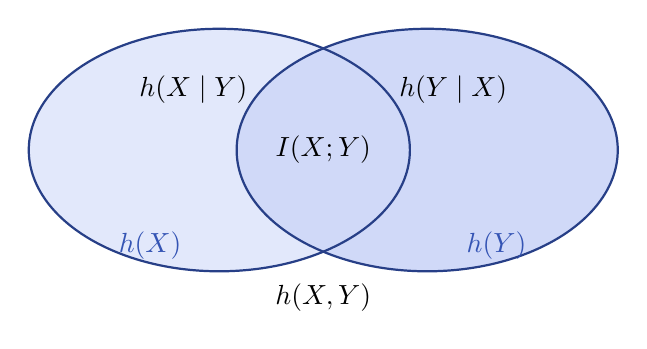
\begin{tikzpicture}[>=stealth, scale=1.1]
  \fill[RoyalBlue!15]  (-1.2,0) ellipse (2.2 and 1.4);
  \fill[RoyalBlue!25]  ( 1.2,0) ellipse (2.2 and 1.4);
  \draw[RoyalBlue!60!black, thick] (-1.2,0) ellipse (2.2 and 1.4);
  \draw[RoyalBlue!60!black, thick] ( 1.2,0) ellipse (2.2 and 1.4);
  \node[RoyalBlue!80!black] at (-2.0, -1.1) {$h(X)$};
  \node[RoyalBlue!80!black] at ( 2.0, -1.1) {$h(Y)$};
  \node at (-1.5, 0.7) {$h(X\mid Y)$};
  \node at ( 1.5, 0.7) {$h(Y\mid X)$};
  \node at ( 0,   0)   {$I(X;Y)$};
  \node at ( 0,  -1.7) {$h(X,Y)$};
\end{tikzpicture}
\end{center}

\noindent 注意：这张图在差熵语境下只能作为关系助记图。连续情形中这些代数关系仍成立，但差熵和条件差熵可能为负，因此不能严格把各部分都理解为非负面积；互信息 $I(X;Y)$ 始终非负。

\subsubsection{典型例题}

\begin{example}
\label{ex:gauss-mi}
\textbf{二维高斯互信息}：设 $(X,Y)$ 服从二维联合高斯分布，边缘方差分别为 $\sigma_x^2$、$\sigma_y^2$，相关系数为 $\rho$。求 $h(X)$、$h(Y)$、$h(X,Y)$、$h(X\mid Y)$、$h(Y\mid X)$ 和 $I(X;Y)$。

\noindent \textbf{解题流程}：\\[2pt]
步骤一：边缘熵直接用一维高斯公式。\\
步骤二：联合熵用多维高斯公式，协方差矩阵 $\Sigma=\bigl(\begin{smallmatrix}\sigma_x^2&\rho\sigma_x\sigma_y\\\rho\sigma_x\sigma_y&\sigma_y^2\end{smallmatrix}\bigr)$，$\det(\Sigma)=\sigma_x^2\sigma_y^2(1-\rho^2)$。\\
步骤三：互信息和条件熵由 $I=h(X)+h(Y)-h(X,Y)$ 导出。

\noindent \textbf{解}：\\[2pt]
\begin{align*}
h(X)  &= \frac{1}{2}\log(2\pi e\sigma_x^2),\\
h(Y)  &= \frac{1}{2}\log(2\pi e\sigma_y^2),\\
h(X,Y) &= \frac{1}{2}\log\bigl[(2\pi e)^2\sigma_x^2\sigma_y^2(1-\rho^2)\bigr]
        = \log(2\pi e\sigma_x\sigma_y\sqrt{1-\rho^2}\,).
\end{align*}
由 $I(X;Y)=h(X)+h(Y)-h(X,Y)$ 得
\[
\boxed{I(X;Y)=-\frac{1}{2}\log(1-\rho^2)}.
\]
条件熵：
\[
h(X\mid Y)=h(X)-I(X;Y)=\frac{1}{2}\log[2\pi e\sigma_x^2(1-\rho^2)],
\qquad
h(Y\mid X)=\frac{1}{2}\log[2\pi e\sigma_y^2(1-\rho^2)].
\]

\noindent \textbf{关键观察}：
\begin{itemize}
  \item $\rho=0$（独立）时 $I(X;Y)=0$，$\rho=\pm1$（完全线性相关）时 $I(X;Y)\to\infty$。
  \item 互信息只依赖于 $|\rho|$，与方差的大小无关——原因是 $h(X)+h(Y)-h(X,Y)$ 中 $\sigma_x^2$ 和 $\sigma_y^2$ 的项恰好对消。方差放大同时增加 $h(X)$ 和 $h(Y)$，但对它们的差没有贡献。
\end{itemize}
\end{example}

\begin{example}
\label{ex:gauss-signal-noise}
\textbf{高斯信号加噪声}：设 $X\sim\mathcal{N}(0,P)$ 为信号，$Z\sim\mathcal{N}(0,N)$ 为独立噪声，$Y=X+Z$。求 $I(X;Y)$。

\noindent \textbf{解}：\\[2pt]
$X$ 与 $Z$ 独立，且均服从高斯分布，故 $(X,Y)$ 为联合高斯。$Y\sim\mathcal{N}(0,P+N)$，
协方差矩阵 $\Sigma_{XY}=\begin{pmatrix}P&P\\P&P+N\end{pmatrix}$。
\[
\det(\Sigma_{XY})=P(P+N)-P^2=PN.
\]
\begin{align*}
h(X)  &= \frac{1}{2}\log(2\pi eP),\\
h(Y)  &= \frac{1}{2}\log[2\pi e(P+N)],\\
h(X,Y) &= \frac{1}{2}\log[(2\pi e)^2 PN].
\end{align*}
\[
I(X;Y)=h(X)+h(Y)-h(X,Y)=\frac{1}{2}\log\frac{P(P+N)}{PN}
      =\boxed{\frac{1}{2}\log\Bigl(1+\frac{P}{N}\Bigr)}.
\]
这就是著名的\textbf{高斯信道容量公式}的基础形式——互信息随信噪比 $P/N$ 对数增长。

\noindent \textbf{直觉理解}：$P/N$ 是信噪比。互信息呈对数增长，是因为高斯熵本身与方差的对数有关；代入后留下 $\log(1+P/N)$。若信噪比从 $s$ 增加到 $2s$，互信息增量为
\[
\frac12\log\frac{1+2s}{1+s}.
\]
只有在高信噪比近似下，这个增量才接近 $\frac12\log 2$。以 2 为底时该近似增量为 $0.5$ bit，以自然对数为底时为约 $0.3466$ nat。
\end{example}

\subsection{题型整理：第四章常见计算}

\begin{methodBox}{连续熵与互信息的通用步骤}
\begin{enumerate}
  \item 先判断随机变量类型：是否高斯？是否独立？
  \item 若是高斯分布，直接套用高斯熵公式，无需积分。
  \item 若涉及线性变换 $Y=AX+\bm{\alpha}$，使用 $h(Y)=h(X)+\log|\det(A)|$。
  \item 求互信息优先用 $I=h(X)+h(Y)-h(X,Y)$，避免直接积分。
  \item 若问题中出现了多个变量，先列出协方差矩阵，再利用 $\det$ 关系简化。
\end{enumerate}
\vspace{2pt}
\noindent \textbf{对应例题}：线性变换见\cref{ex:gauss-linear-transform} 和 \cref{ex:gauss-orthogonal}；高斯互信息见\cref{ex:gauss-mi}；信号加噪声见\cref{ex:gauss-signal-noise}。
\end{methodBox}

\begin{methodBox}{最大熵题的解题思路}
题目通常给出约束条件（幅度范围或方差/协方差），问何种分布熵最大、最大值是多少。
\begin{itemize}
  \item 先判断约束类型：限峰值（区间）还是限平均功率（方差）。
  \item \textbf{限峰值} $\to$ 均匀分布，直接代入 $h=\log(b-a)$ 或 $\sum\log(b_i-a_i)$。
  \item \textbf{限功率} $\to$ 高斯分布，代入 $h=\frac{1}{2}\log(2\pi e\sigma^2)$ 或多维公式。
  \item 多维实用技巧：独立分量时用 $\prod\sigma_i^2$，相关分量时用 $\det(\Sigma)$。
\end{itemize}
\end{methodBox}

\begin{warningBox}{常见混淆}
不要混淆：
\begin{itemize}
  \item 离散熵 $H(X)\ge 0$ 与差熵 $h(X)$ 可正可负——差熵不是信息量的绝对度量。
  \item 最大熵的约束条件：限峰值对应均匀分布，限功率对应高斯分布。考试中经常反过来问——看到均匀分布要想到幅度受限，看到高斯要想到功率受限。
  \item $I(X;Y)$ 在连续情形下仍非负，且对 $X$、$Y$ 分别作可逆变换时保持不变；但中间步骤的 $h(X)$、$h(Y)$ 可能会在变换中改变。
\end{itemize}
\end{warningBox}

\subsection{公式速查表}

{\scriptsize
\begin{tabularx}{\textwidth}{@{}l>{\raggedright\arraybackslash}X>{\raggedleft\arraybackslash}p{1.8em}@{}}
\toprule
\textbf{类别} & \textbf{公式} & \textbf{编号} \\
\midrule
\textcolor{Red}{差熵定义} & $\textcolor{Red}{h(X)=-\int_{\mathbb{R}} p(x)\log p(x)\,\mathrm{d}x}$ & (1) \\
联合差熵 & $h(X^N)=-\int_{\mathbb{R}^N} p(\bm{x})\log p(\bm{x})\,\mathrm{d}\bm{x}$ & (2) \\
条件差熵 & $h(X\mid Y)=-\iint_{\mathbb{R}^2} p(x,y)\log p(x\mid y)\,\mathrm{d}x\mathrm{d}y$ & (3) \\
\midrule
\textcolor{Red}{一维高斯熵} & $\textcolor{Red}{h(X)=\frac12\log(2\pi e\sigma^2)}$ & (4) \\
\textcolor{Red}{多维高斯熵} & $\textcolor{Red}{h(X^N)=\frac{N}{2}\log[2\pi e\det(\Sigma)^{1/N}]}$ & (5) \\
\midrule
\textcolor{Red}{线性变换} & $\textcolor{Red}{h(Y)=h(X)+\log|\det(A)|}$ & (6) \\
\midrule
\textcolor{Red}{限峰值最大熵} & $\textcolor{Red}{h(X)\le\log(b-a)}$（均匀分布） & (7) \\
\textcolor{Red}{限功率最大熵} & $\textcolor{Red}{h(X^N)\le\frac{N}{2}\log[2\pi e\det(\Sigma)^{1/N}]}$（高斯分布） & (8) \\
\midrule
\textcolor{Red}{连续相对熵} & $\textcolor{Red}{D(p\|q)=\int_{\mathbb{R}} p(x)\log\frac{p(x)}{q(x)}\,\mathrm{d}x\ge 0}$ & (9) \\
\midrule
\textcolor{Red}{连续互信息} & $\textcolor{Red}{I(X;Y)=\iint_{\mathbb{R}^2} p(x,y)\log\frac{p(x,y)}{p(x)q(y)}\,\mathrm{d}x\mathrm{d}y}$ & (10) \\
 & $\textcolor{Red}{I(X;Y)=h(X)+h(Y)-h(X,Y)}$ & (11) \\
\textcolor{Red}{高斯互信息} & $\textcolor{Red}{I(X;Y)=-\frac12\log(1-\rho^2)}$ & (12) \\
\textcolor{Red}{信号+噪声} & $\textcolor{Red}{I(X;Y)=\frac12\log\bigl(1+\frac{P}{N}\bigr)}$ & (13) \\
\bottomrule
\end{tabularx}
}

\subsection{本章小结}
\begin{remarkBox}{第四章知识脉络}
本章将信息度量从离散推广到连续，核心思想是「离散化取极限」：

\textbf{学习提示}：
\begin{itemize}
  \item 考试中绝大多数连续熵的计算题都可以用高斯熵公式直接写出答案，不需要积分。
  \item 线性变换公式 $h(Y)=h(X)+\log|\det(A)|$ 是处理坐标变换的首选工具。
  \item 最大熵定理是概念题的高频考点——记住：限峰值 $\to$ 均匀，限功率 $\to$ 高斯。
  \item 连续互信息的性质与离散完全一致，差熵的可加性、不增性也保持不变；第二章的关系链仍可用，但 Venn 图只宜作为助记。
\end{itemize}

\begin{center}
\small
\begin{tikzpicture}[>=stealth, node distance=2.2cm]
  \node[draw, fill=MidnightBlue!10, rounded corners, font=\bfseries] (A) {连续信源};
  \node[draw, fill=RoyalBlue!10, rounded corners, font=\bfseries] (B) [below of=A] {离散化 + 取极限};
  \node[draw, fill=SeaGreen!10, rounded corners, font=\bfseries] (C) [below of=B, xshift=-2.8cm, align=center] {差熵 $h(X)$\\（相对度量，可负）};
  \node[draw, fill=SeaGreen!10, rounded corners, font=\bfseries] (D) [below of=B, xshift=2.8cm, align=center] {相对熵 $D(p\|q)$\\（$\ge 0$，与离散一致）};
  \node[draw, fill=Orange!10, rounded corners, font=\bfseries] (E) [below of=C, align=center] {高斯熵\\$h=\frac12\log(2\pi e\sigma^2)$};
  \node[draw, fill=Orange!10, rounded corners, font=\bfseries] (F) [below of=D, align=center] {最大熵定理\\均匀 / 高斯};
  \node[draw, fill=Red!10, rounded corners, font=\bfseries] (G) [below of=E, xshift=2.8cm, align=center] {连续互信息\\$I(X;Y)\ge0$\\可逆变换不变};

  \draw[->, thick] (A) -- (B);
  \draw[->, thick] (B) -- (C);
  \draw[->, thick] (B) -- (D);
  \draw[->, thick] (C) -- (E);
  \draw[->, thick] (D) -- (F);
  \draw[->, thick] (E) -- (G);
  \draw[->, thick] (F) -- (G);
\end{tikzpicture}
\end{center}
\end{remarkBox}

\subsection{本章要求}
第四章学习重点：
\begin{itemize}
  \item 理解连续随机变量的\textbf{离散化取极限}思想，掌握\textbf{差熵}的定义和计算；
  \item 掌握\textbf{一维和多维高斯分布}的差熵公式；
  \item 掌握\textbf{线性变换}下差熵的变化规律（$h(Y)=h(X)+\log|\det(A)|$）；
  \item 熟记\textbf{限峰值最大熵定理}（均匀分布）和\textbf{限平均功率最大熵定理}（高斯分布）；
  \item 掌握连续随机变量的\textbf{平均互信息}及其性质，能利用 $I=h(X)+h(Y)-h(X,Y)$ 进行计算；
  \item 理解差熵与离散熵的异同：非负性、绝对度量、变换性质。
\end{itemize}
